

\chapter{Pr\'{e}sentation de mon environnement \`{a} SAP}


\section{Présentation de l'équipe}




\begin{figure}[h!]
  \centering
      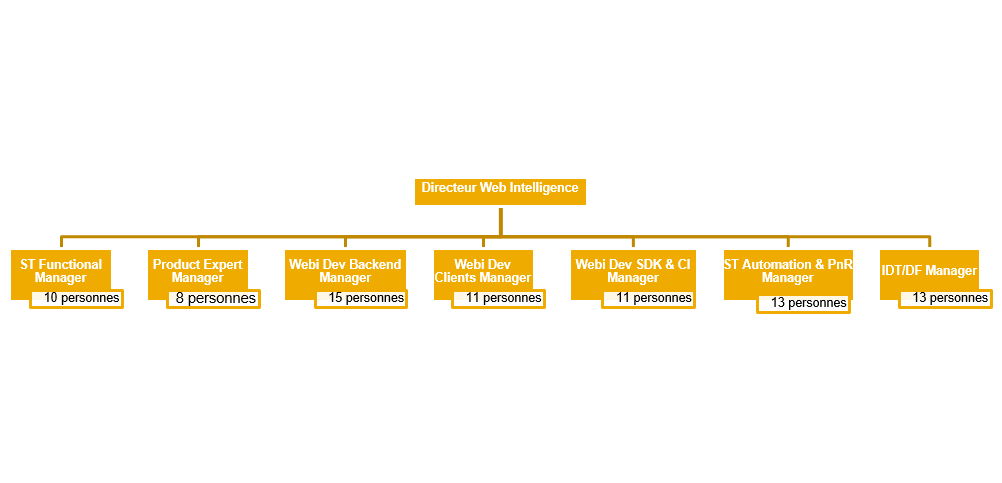
\includegraphics[width=1.2\textwidth]{images/allRaphaelTeam.png}
  \caption{\'{E}quipe Web Intelligence}
	\label{figure:}
\end{figure}








\section{Sa mission}

L'\'{e}quipe transversale fournit les services transversaux, faisant appel à des compétence spécifiques.\\
Particuli\`{e}rement foculis\'{e}e sur le test coverage\index{Test coverage}, différentes missions ce l'\'{e}quipe transverse peuvent être divisées en cinq catégories\footnote{se reporter à l'organigramme page \pageref{pdf:org}} :\\

\begin{description}
	\item[Tests fonctionnels] Assurés par 3 personnes, leurs tests portent sur le SDK de Web Intelligence. 
	\item[Tests automation] Assurés par 3 personnes, leur mission est d'ajouter les tests implémentés et de les mettre en production, quelque soit le test (son Framework ou le langage utilisé).
	\item[Benchmark] Assurés par 3 personnes, ils s'occupent des tests de benchmark, autrement dit, les tests de performance, de stabilité et de scalabilité. Ils sont parfois appelés à implémenter quelques codes mais utilises, en règle général, des logiciels pour générer des charges, ouvrir de multiples documents, installer le produit, répéter la même action des centaines de fois, \ldots. Ils sont aussi en charge des acceptances, autrement dit la validation de tous les tests existants afin de certifier que le produits et fonctionnel.
	\item[Mise en production] Sa mission est de mettre en production les produits développées par et pour les équipes SAP. Une personnes s'occupe de cette mission.
	\item[Développement] Développement d'outils internes et d'outils de reporting, construction de rapport WebI. Une personnes s'occupe de cette mission.
\end{description}






